\documentclass[a4paper, 12pt]{article}
% math symbols
\usepackage{amssymb}
\usepackage{amsmath}
\usepackage{mathrsfs}
\usepackage[shortlabels]{enumitem}
\usepackage{mathseries}
\usepackage[12pt]{moresize}
\usepackage[style = alphabetic, maxbibnames = 99, backend = biber]{biblatex}
\addbibresource{references.bib}

\usepackage[margin = 2cm]{geometry}

\tolerance = 1000
\emergencystretch = 0.74cm



\pagestyle{empty}
%\parindent = 0mm

\let\D\undefined

\newauthor{ds}{Dmitry}{red!20}

\notesmode

\begin{document}
%    \pagestyle{empty}


\begin{tikzpicture}[remember picture, overlay]
    \node[
        shape = rectangle,
        minimum height = \paperheight,
        minimum width = \paperwidth,
        anchor = south west,
        fill = olive!5]
        (sheet) at (current page.south west) {};
    \tikzset{shift = {(sheet.center)}}
    \node at (0, -2) {
        \HUGE
        \begin{tabular}{c}
            \textsc{Теория информации}\\
            \huge Конспект лекций
        \end{tabular}
    };

    \node[inner sep = 0pt, opacity = 0.5] at (6, 10.5){
        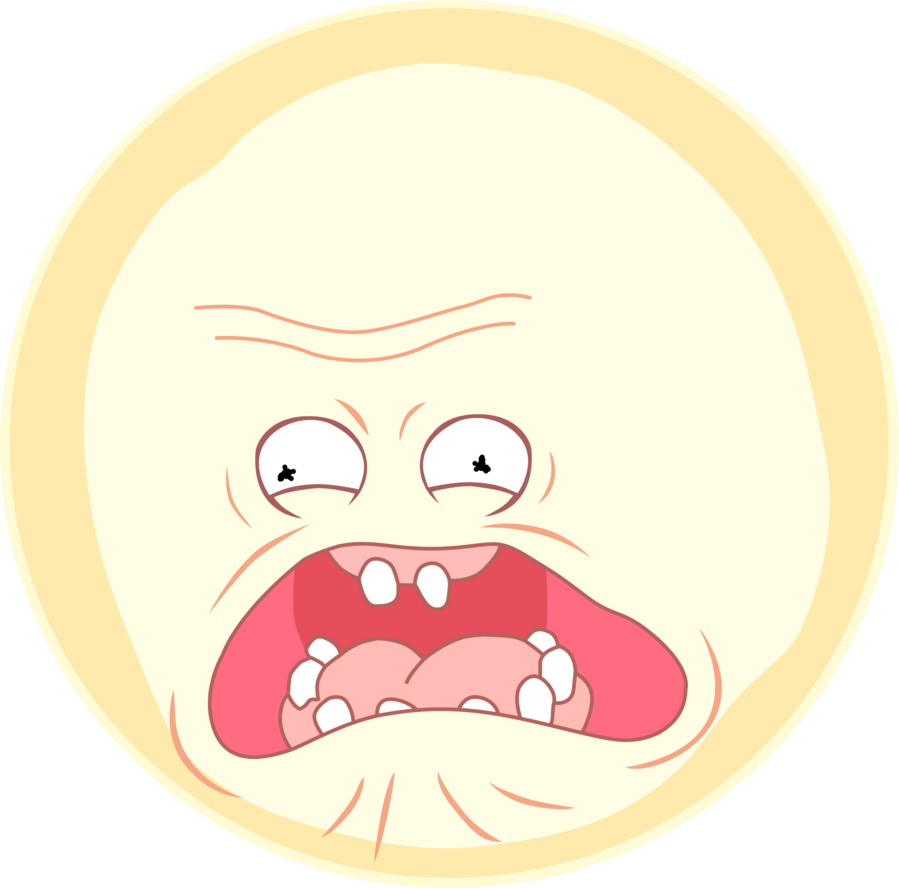
\includegraphics[width = 0.27\textwidth] {pics/sun.png}
    };


    \begin{scope}[shift = {(0, 3)}]
        \node[inner sep = 0pt, opacity = 0.5] at (-5, 0){
            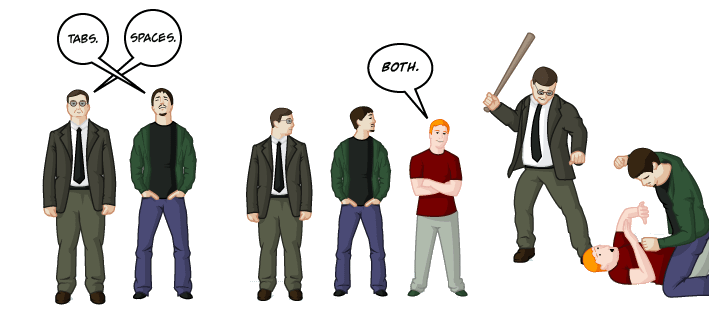
\includegraphics[width = 0.4\textwidth] {pics/tabs-spaces.png}
        };
        \node[inner sep = 0pt, opacity = 0.5] at (-5, -2.3){
            \textsc{Коммуникационная сложность}
        };
        \node[inner sep = 0pt, opacity = 0.5] at (5, 0){
            
\includegraphics[width = 0.4\textwidth] {pics/bender.png}
        };
        \node[inner sep = 0pt, opacity = 0.5] at (5, -2.3){
            \textsc{Колмогоровская сложность}
        };
    \end{scope}

    \begin{scope}[shift = {(0, -8)}]
        \node[inner sep = 0pt, opacity = 0.5] at (0, 0){
            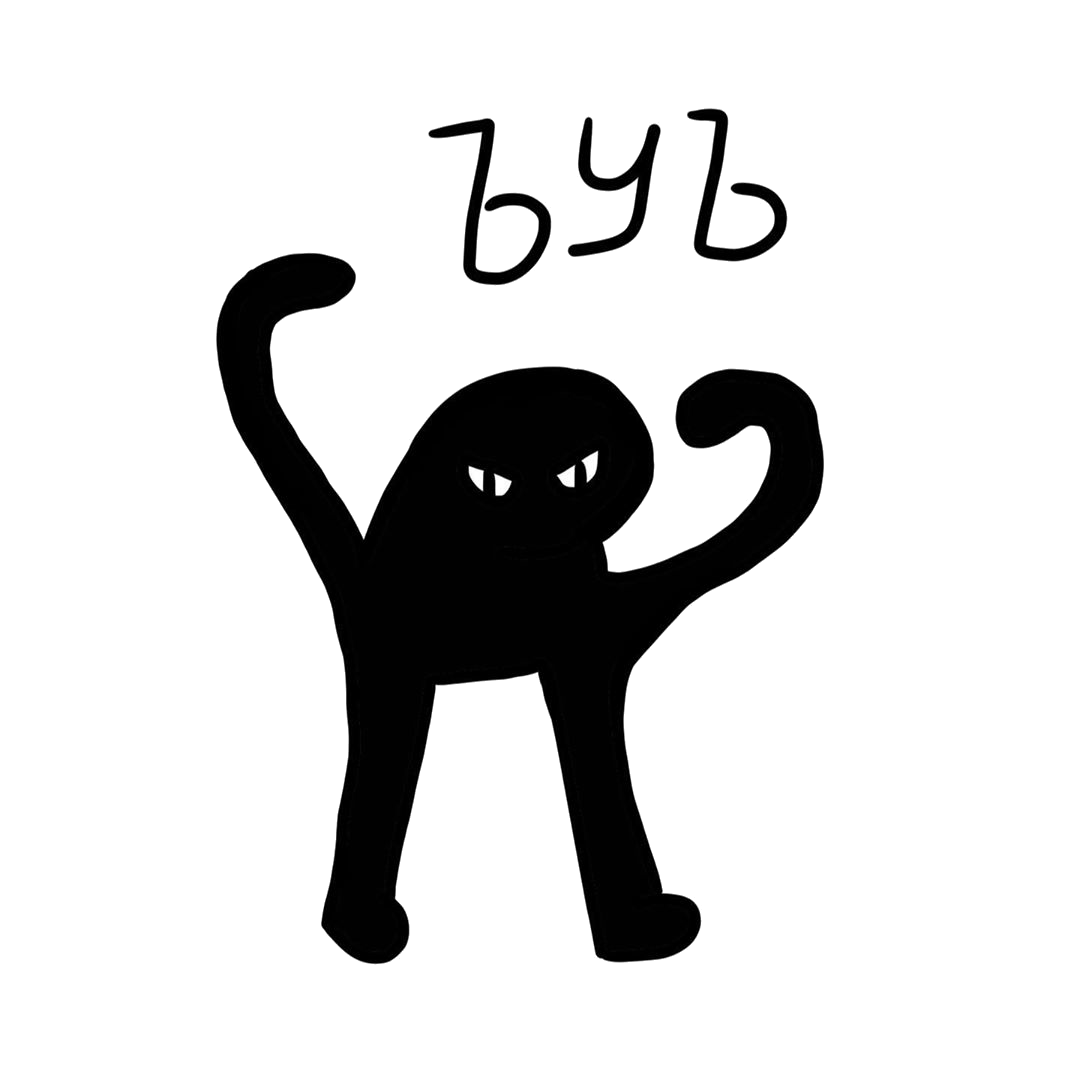
\includegraphics[width = 0.5\textwidth] {pics/uuu.png}
        };
        \node[inner sep = 0pt, opacity = 0.5] at (0, -4.2){
            \textsc{Теория кодирования}
        };
    \end{scope}


%    \pic[scale = 1.6] at (-3.5, -5) {tikzart-gun};

%    \pic[scale = 1.6] at (7, -9) {tikzart-bunny};
%    \pic[scale = 1.6] at (-5, 5) {tikzart-bunny};
%    \pic[scale = 1.6, rotate = 40] at (-5, -8) {tikzart-bunny};
%    \pic[scale = 1.6, rotate = -10, xscale = -1] at (6, 1) {tikzart-bunny};
%    \pic[scale = 1.6, rotate = 30, xscale = -1] at (8, 9) {tikzart-bunny};

%    \draw[platform] (\paperwidth / 2, -12.02) -- ++(-\paperwidth, 0);

%    \foreach \i in {0, 1, ..., 4}{
%        \pic[scale = 4] at (-5 + 1.8 * \i, -12) {tikzart-train};
%        \draw (-3.2 + 1.8 * \i, -11.7) -- ++(-0.2, 0);
%    }
%    \pic[scale = 4] at (-5 + 1.8 * 5, -12) {tikzart-trainhead};
\end{tikzpicture}


\clearpage


    \tableofcontents
    \clearpage

    \setmathstyle{2020}{Коммуникационная сложность}{\thepage}

    \author{Авторы конспекта: Пётр Смирнов, Анастасия Софронова\\ Лектор: Дмитрий Соколов}
%{\let\newpage\relax\maketitle}




    Курс состоит из 15 лекций:
\begin{itemize}
    \item 8 лекций, записанных \href{https://www.lektorium.tv/node/36683}{Лекториумом};
    \item 7 лекций, проведённых в Zoom: 6 из них есть на \href{https://www.youtube.com/playlist?list=PLKXEsFnBcT5ABaSHIAe0lKDnL8CLzmn5z}{YouTube}, недостающая лекция за 15.04.2020 есть в  \href{https://vk.com/videos-193571461?section=album_34}{VK}.
\end{itemize}

В этом конспекте Петром записаны Лекториум-лекции 1--8 и Zoom-лекции 1 и 2. При этом Лекториум-лекция 8 дана как ссылка на другой конспект на русском языке, а Zoom-лекция 1 записана не очень подробно.

Начиная с Zoom-лекции 3 (product distributions), записывала Анастасия.

В лекциях было много неточностей, особенно ошибок в вычислениях "--- мы постарались их исправить (какие-то самостоятельно, какие-то в результате обсуждения на консультации).

Пишите об ошибках любого уровня "--- как об опечатках и языковых ошибках, так и о содержательных проблемах.

Являются ли теории $Th(\mathbb{Z}, <, =)$ и $Th(\mathbb{Q}, <, =)$ эквивалентными? Если да, то докажите, если нет, то предъявите
пример разделяющей формулы.

\task{
    Пусть $\sigma$~--- сигнатура линейных порядков. Существует ли такая замкнутая $\sigma$-формула
    $\varphi$, что $\varphi$ истинна во всех интепретациях $\sigma$, являющихся линейными порядками
    мощности $m$ и только в них (возможно еще в каких-то бесконечных интерпретациях), где $m$~---
    произвольное составное число.
}    
\task{
    Пусть $\Kolm(x) = s$, оцените $\Kolm(x x^1 x^2 x^3 \dots x^{|x|})$, где $x^i$~--- строка $x$ с
    инвертированным битом на позиции $i$.
}    

%Предъявите аксиоматику теории $Th(\mathbb{Z}, <, =)$.
%\begin{definition*}
    Пусть $X \coloneqq \{x_1, \dots, x_n\}$~--- множество булевых переменных, а $\mathcal{O}$~---
    конечное множество. Будем говорить, что \deftext{линейная ветвящаяся программа}~--- это направленный
    ациклический граф, с одним истоком. Каждая внутренняя вершина этого помечена функцией вида $a_0
    \oplus a_1 x_1 \oplus a_2 x_2 \oplus \dots \oplus a_n x_n$, где $a_{i} \in \{0, 1\}$, а каждый сток
    элементом $\mathcal{O}$. При этом из каждой внутренней вершины исходит ровно два выходящих ребра:
    помеченное нулем и помеченное единицей.

    Будем считать, что ветвящаяся программа $B$ считает функцию $f_{B}\colon \{0, 1\}^n \to
    \mathcal{O}$. Каждое значение входных переменных $z \in \{0, 1\}^n$ индуцирует путь из истока в сток
    естественным образом. Если путь заканчивается в вершине с пометкой $o \in \mathcal{O}$, то мы
    считаем, что $f_B(z) \coloneqq o$.
\end{definition*}

\task{
    Покажите, что существует функция, для которой любая ветвящаяся программа имеет размер не менее
    $\frac{2^{n}}{\poly(n)}$. 
}
%Покажите, что следующие теории не являются изоморфными $Th(\mathbb{N} + \mathbb{N}, <, =)$ и $Th(\mathbb{N}, <, =)$.
%%2020-03-25
\section{Улучшенная верхняя оценка для \texorpdfstring{$\R^{pub}(\GT)$}{R[pub](GT)}}

По теореме~\ref{R-pub(GT) simple} $\R^{pub}(\GT)\leqslant \O(\log n\cdot \log\log n)$. Докажем лучшую оценку:
\begin{theorem}
$\R^{pub}(\GT)\leqslant \O(\log n)$.
\end{theorem}
\begin{proof}
Потребуем ошибку в протоколе для $\EQ$ не более $\frac{1}{100}$.
Идём по дереву бинпоиска, оказываясь в вершине, перепроверяем, всё ли ок. Если не ок, поднимаемся наверх по ребру.

Следим за величиной <<расстояние до правильного листа>>.
Покажем, что через $100\log n$ итераций с большой вероятностью будет нулём: по неравенству Маркова вероятность ошибки $\leqslant \frac{1}{100}$.

Можно воспользоваться оценками Чернова, тогда вероятность ошибки $\leqslant 2^{-\Omega(\log n)} = \O\left(\frac{1}{n}\right)$. Это можно использовать для правильного понижения ошибки. \mycomment{\textcolor{red}{На лекции на 34:20 говорится, что в оценках Чернова квадрат от числа итераций (и получается ошибка $\O(n^{-\log n})$) "--- это странно. Что именно здесь имеется в виду про понижение ошибки, я не очень понял.}}
\end{proof}

\section{Нижняя оценка на \texorpdfstring{$\DPLL_\oplus$}{DPLL(⊕)} через \texorpdfstring{$\R^{pub}(\Search_\phi)$}{R[pub](Search(φ))}}

\begin{theorem}
\label{DPLL-oplus and Search}
Пусть $T = \DPLL_{\oplus}(\phi)$.
Тогда $\R^{pub}(\Search_{\phi}) \leqslant \log T\log\log T$.
\end{theorem}
\begin{proof}
Как в доказательстве теоремы~\ref{DPLL and Search} для обычного $\DPLL$, только теперь надо проверить выполненность системы линейных уравнений.
Чтобы проверить, выполняется ли система, нужно проверить $k$ равенств.
Делаем это с помощью протокола для $\EQ$ с вероятностью ошибки не более $1/\log T$.
\end{proof}
\begin{remark}
Можно избавиться от $\log\log T$ аналогично тому, как мы сделали это в $\GT$.
Тогда получим $\R^{pub}(\Search_{\phi}) \leqslant \log T$, то есть $T\geqslant 2^{\R^{pub}(\Search_\phi)}$.
\end{remark}
\begin{proof}
Оставлено как упражнение.
\end{proof}
%\mytitle{7 (на 19.10)}

\newcommand{\dom}[2]{\left[\frac{#1}{#2}\right]}

\begin{task}
	Покажите, что универсальный предикат для класса одноместных разрешимых предикатов не является разрешимым.
\end{task}


\begin{task}
    Докажите, что следующие функции являются примитивно рекурсивными:
    \begin{enumerate}[topsep = 0pt, itemsep = -1ex]
        \item [а)] $x^y$;
        \item [б)] $x!$;
        \item [в)] Покажите, что усеченное вычитание $x \dot{-} y$, которое равняется $x - y$, если $x \ge y$ и нулю иначе,
			является примитивно рекурсивным; 
    	\item [г)] $min(x, y)$;
        \item [д)] $max(x, y)$;
    \end{enumerate}
\end{task}


Множество $S \subseteq \mathcal{N}^k$ называется примитивно рекурсивным, если его характеристическая функция примитивно
рекурсивна.

\begin{task}	
    \begin{enumerate}[topsep = 0pt, itemsep = -1ex]
        \item [а)] Покажите, что множество $S \subseteq \mathcal{N}^k$ примитивно рекурсивное, тогда и только тогда, когда оно
			есть множество нулей некоторой примитивно-рекурсивной функции;
        \item [б)] покажите, что объединение, пересечение и дополнение примитивно рекурсивных множеств является примитивно
			рекурсивным.
        \item [в)] покажите, что предикат $x = y$ примитивно рекурсивен;
        \item [г)] покажите, что предикат $x > y$ примитивно рекурсивен.
    \end{enumerate}
\end{task}


\begin{task}
    Пусть отношение $R(x, y)$ задает примитивно рекурсивное множество (т.е. множество $\{(x, y) \mid R(x, y) = 1\}$), докажите,
    что отношения $S(x, z) = \exists (y \le z) R(x, y)$ и $T(x, z) = \forall (y \le z) R(x, y)$ также задают примитивно
    рекурсивные множества.
\end{task}

\begin{task}
    Докажите, что существует такое подмножество натуральных чисел, что его симметрическая разность с любым перечислимым множеством
    имеет бесконечный размер.
\end{task}



\breakline

\begin{ptask}{21}
	Задача Поста состоит в следующем: есть доминошки $n$ видов $\dom{s_1}{t_1}, \dom{s_n}{t_n}$, $s_i$ и $t_i$~--- конечные
    строки, есть неограниченный запас доминошек каждого вида, доминошки переворачивать нельзя. Требуется определить, можно ли
    составить несколько доминошек так, чтобы в верхней и нижней их половине читалась одна и та же строка, такие последовательности
    доминошек будем называть согласованными. Докажите, что задача Поста алгоритмически неразрешима.
\end{ptask}


\begin{ptask}{31}
	Обозначим через $K(x)$ минимальное такое число $n$, что алгоритм с номером $n$ (номер алгоритма~--- это номер его текста, при
    этом строчки упорядочиваются сначала по длине, потом по алфавиту) на входе $0$ входе печатает $x$ и останавливается. Докажите,
    что $K(x)$ не является вычислимой функцией.
\end{ptask}

\begin{ptask}{32}
	Пусть предикат $A(n, x)$ обладает таким свойством: для любого разрешимого предиката $R(x)$ найдется такое натуральное число
    $r$, что $A(r, x) = R(x)$ для всех $x$. Покажите, что предикат $A$ не разрешим.
\end{ptask}

%%2020-04-01

\chapter{Distributional protocols}
\section{Определения и свойства}
Пусть для каждого входа $(x, y)$ задана его вероятность $\mu(x, y)$.
Distributional protocol "--- \emph{детерминированный} протокол, который решает правильно задачу на всех входах, кроме доли, имеющей меру не более $\eps$.
Сложность протокола $\D^\mu_\eps(f)$ "--- это высота дерева.

\begin{theorem}
$\R^{pub}_\eps(f) = \max_{\mu} \D^{\mu}_\eps (f)$
\end{theorem}
\begin{proof}
$\geqslant$: Для любого $\mu$ мы можем из $\R_\eps$  получить протокол: выберем наилучшие случайные биты. У них будет ошибка не более меры $\eps$, иначе есть вход, у которого ошибка больше $\eps$ в протоколе $\R_\eps$.

$\leqslant$. Пусть $c = \max_{\mu} \D^{\mu}_\eps (f)$. Будем использовать минимакс-теорему (формулировку см. ниже).
Строки матрицы помечены всеми возможными входами $(x, y)$.
Столбцы помечены всеми детерминированными протоколами сложности не более $c$.
В клетке ставим $1$, если протокол верно работает на этом входе, и $0$ иначе.

Рассмотрим распределение на входах $p$ и вероятностный протокол $\Pi$, являющийся распределением $q$ на детерминированных протоколах. Тогда $p^TAq$ "--- это вероятность верного ответа $\Pi$ на распределении на входах $p$.

Мы знаем, что для любого распределения на входах $p$ найдётся даже детерминированный протокол с ошибкой не более $\eps$, поэтому $\min_p\max_q p^TAq\geqslant 1-\eps$.

По минимакс-теореме $\max_q\min_p p^TAq\geqslant 1-\eps$. То есть существует вероятностный протокол $\Pi$ такой, что какое бы распределение на входах не выбрать, вероятность верного ответа хотя бы $1-\eps$. Выбирая распределения, сконцентрированные на одном входе, получаем требуемое.
\end{proof}

\begin{theorem}[Минимакс-теорема, фон Нейман, 1928]
Пусть $A$ "--- матрица, Алиса выбирает строку, Боб выбирает столбец, Алиса получает число денег, написанное в клетке на пересечении.

Пусть теперь выбираем вероятности $p_i$ для строк и $q_j$ для столбцов. $\E[\text{выигрыш}] = p^TAq$.

Тогда $\max_{p} \min_{q} p^TAq  = \min_{q} \max_{p} p^TAq$.
\end{theorem}

\mycomment{\textcolor{red}{TODO: Добавить сюда комментарий про неправильную формулировку.}}

Нижние оценки на $\R(f)$ можно получать, выбирая распределение $\mu$ и доказывая нижнюю оценку.
Все известные нижние оценки на $\R(f)$, кроме лифтинга, так и устроены.

\section{Discrepancy}
Discrepancy "--- обобщение техники Rectangle Size. Пусть задано распределение на входах $\mu$.

\begin{definition}
Discrepancy прямоугольника $R$ "--- это $\disc_{\mu}(f, R) = \left|\mu(R\cap f^{-1}(0)) - \mu(R\cap f^{-1}(1)\right|$.

Discrepancy функции $f$ "--- это $\disc_\mu(f) = \max_R \disc_{\mu}(f, R)$ по всем прямоугольникам $R$.
\end{definition}

\begin{theorem}
$\D^\mu_{1/2-\eps}(f) = \Omega\left(\log\left(\frac{2\eps}{\disc_{\mu}(f)}\right)\right)$
\end{theorem}
\begin{proof}
Рассмотрим прямоугольник $R_i$ листа $l_i$. Пусть вероятность ошибки этого листа есть $\mathrm{err}_i$ (она не больше $\mu(R_i)/2$). Тогда $\disc(R_i) = (\mu(R_i) - \mathrm{err}_i) - \mathrm{err}_i = \mu(R_i) - 2\mathrm{err}_i$.

Рассмотрим $\sum_i \disc(R_i)$. С одной стороны, это $\sum (\mu(R_i) - 2\mathrm{err}_i) = 1 - 2\mathrm{err} = 1 - 2(1/2 - \eps) = 2\eps$.

С другой стороны, слагаемых в сумме $2^\D$, у каждого $\disc$ не больше $\disc(f)$. Поэтому $2\eps \leqslant 2^\D\cdot \disc(f)$, откуда $\D\geqslant \log\left(\frac{2\eps}{\disc(f)}\right)$.

\mycomment{На лекции предлагалось посмотреть на большой прямоугольник в листе, но доказательство было оставлено как упражнение. У меня не получилось реализовать этот план, оценка получается слабее.}

%Выберем самый большой прямоугольник в листе, пусть он размера $s$. Тогда всего листьев хотя бы $1/s$, тогда высота протокола хотя бы $\log(1/s)$.

%Если прямоугольник имеет $\disc = d$, то в нём хотя бы (по мере) $(s - d)/2$ и нулей, и единиц. Значит, $(s-d)/2\le \eps$, то есть $.

%Надо показать, что прямоугольник имеет размер не больше $\frac{2\eps}{\disc_{\mu}(f)}$.  этого прямоугольника не более $\disc_\mu(f)$, поэтому и нуле

%Если $\disc$ маленький, а прямоугольник в листе большой, то ошибаемся слишком много.
\end{proof}

\begin{theorem}
$\disc_{uni}(\IP) \leqslant 2^{-n/2}$.
\end{theorem}
\begin{proof}
Рассмотрим $\pm 1$-матрицу $A$ для $\IP$.

Рассмотрим прямоугольник $R = S\times T$. $\disc(\IP, R) = \left|\sum_{(x,y)\in R} (-1)^{\langle x, y\rangle}\right| / 2^{2n}$.

Числитель:
$|\One^T_S\cdot A\cdot \One_T| \leqslant
\lVert A\rVert_2 \lVert \One_S\rVert_2 \lVert \One_T\rVert_2 \leqslant
\lVert A\rVert_2 \sqrt{|S||T|} = 
\lVert A\rVert_2 \sqrt{|R|}
$.

$A^2 = 2^{n} E$ "--- проверили явно, см. второе доказательство теоремы~\ref{rk(M-IP) lower bound}.
Поэтому $\lVert A^2\rVert_2 = 2^n$, и $\lVert A\rVert_2=2^{n/2}$.

Итого числитель $\leqslant 2^{n/2}\sqrt{|R|} \leqslant 2^{3n/2}$, что и требовалось доказать.
\end{proof}

Из этого получаем нижнюю оценку на $\R(\IP)$:

\begin{theorem}
$\R(\IP)\geqslant \Omega(n)$.
\end{theorem}

Для $\DISJ$ доказать нижнюю оценку таким способом не получится:

\begin{proposition}
Для любого распределения $\mu$ $\disc_\mu(\DISJ)\geqslant \frac{1}{2n} - \frac{1}{2n^2}$.
\end{proposition}

То есть нижняя оценка на коммуникацию получится разве что логарифмическая.

\begin{proof}
Посмотрим на всю матрицу $M$.
Пусть $\disc(\DISJ, M) < \frac{1}{n}$.
Тогда мера нулей хотя бы $\frac{1}{2}-\frac{1}{2n}$.
Но у нулей есть покрытие $n$ 0-прямоугольниками.
Тогда какой-то из них имеет меру не менее $(\frac{1}{2}-\frac{1}{2n})/n$ и такое же $\disc$.
\end{proof}

\begin{theorem}[Babai et al.; 1986]
$\D^{uni}_{\eps}(\DISJ^{\leqslant \sqrt{n}}_n) = \Omega(\sqrt{n})$
\end{theorem}
\begin{proof}
Пусть $\eps < 1/100$.

Будем рассматривать (почти 1)-прямоугольники.
Пусть в прямоугольнике $S\times T$ не более $\eps$ нулей.
Покажем, что либо $\mu(S)\leqslant 2^{-c\sqrt{n}}$, либо $\mu(T)\leqslant 2^{-c\sqrt{n}}$.

(Продолжение в следующий раз.)
\end{proof}

Из этого получаем:

\begin{theorem}
$\R(\DISJ) = \Omega(\sqrt{n})$.
\end{theorem}

Для product-распределений это является и верхней оценкой.
%(???) связь недетерминированных и вероятностных
%\mytitle{10 (на 20.04)}

\begin{task}
    Докажите, что язык булевых формул с ровно одним выполняющим набором ($\USAT$):
    \begin{enumerate}[topsep = 0pt, itemsep = -1ex]
        \item [а)] $\coNP$-трудным;
        \item [б)] лежит в $\P^{\NP}$.
    \end{enumerate}
\end{task}

Определим класс $\UP$. $L \in \UP$, если существует такая недетерминированная машина
Тьюринга $M$, что для любого $x$ выполнено: $M(x) = L(x)$ и существует не более одной
подсказки, которая принимается машиной $M$.

\begin{task}
    Докажите, что: 
    \begin{enumerate}[topsep = 0pt, itemsep = -1ex]
        \item [а)] язык простых чисел лежит в классе $\UP$;
        \item [б)] если $\USAT \in \UP$, то $\NP = \coNP$.
    \end{enumerate}
\end{task}

\begin{task}
    Покажите, что существует такой оракул $A$ и язык $L \in \NP^A$, что $L$ не
    сводится по Тьюрингу к $3\SAT$, даже если сведение может использовать оракул $A$.
\end{task}

\breakline

\begin{ptask}{26}(подсказка: $\NEXP^{\NP} vs. \NEXP$)
    Докажите, что если $\P = \NP$, то существует язык из $\EXP$, схемная сложность которого не меньше $\frac{2^n}{10 n}$.
\end{ptask}

\begin{ptask}{40}
    Докажите, что если $\NP \subseteq \BPP$, то $\NP = \RP$.
\end{ptask}

\begin{ptask}{44}
    Покажите, что:
	\begin{enumerate}[topsep = 0pt, itemsep = -1ex]
        \item [а)] если $\BPTime[f(n)] = \BPTime[g(n)]$, то $\BPTime[f(h(n))] = \BPTime[g(h(n))]$, где $f, g, h$~---
			конструктивные по времени, $f(n), g(n) \ge \log n$, $h(n) \ge n$~--- возрастающая функция;
        \item [б)] $\DTime[f(n)] \subseteq \BPTime[f(n)] \subseteq \DTime[2^{O(f(n))}]$;
        \item [в)] $\BPP \subseteq \BPTime[n^{\log n}] \subsetneq \BPTime[2^n]$.
    \end{enumerate}
\end{ptask}

\begin{ptask}{45}
    Определим язык $\lang{QNR} = \{(y, m) \mid \text{$y$ не является квадратичным вычетом по модулю $m$}\}$, докажите, что
    $\lang{QNR} \in \IP$.
\end{ptask}

\begin{ptask}{46}
    $\BPL_H$~--- это класс языков, для которых существует вероятностная машина Тьюринга $M$, которая использует логарифмическую
    память, останавливается с вероятностью $1$, и для всех $x$ выполняется, что $\Pr[M(x) = L(x)] \ge \frac{2}{3}$. Покажите, что
    $\BPL_H \subseteq \P$.
\end{ptask}

\begin{ptask}{49}
    Покажите, что:
    \begin{enumerate}[topsep = 0pt, itemsep = -1ex]
        \item [в)] если граф представляет собой шахматную доску с выбитыми клетками
            (вершины~--- клетки, ребра соединяют соседние клетки), то существует
            полиномиальный алгоритм, который считает число полных паросочетаний
            (подсказка: иногда вес ребра удобно взять комплексным).
    \end{enumerate}    
\end{ptask}


\begin{ptask}{51}
    Существует вариант класса $\MA$ с односторонней ошибкой. $L \in \MA_1$, если существует такая полиномиальная вероятностная
    машина $V$ и полином $p$, что если $x \in L$, то найдется такая строка $y \in \{0, 1\}^{p(n)}$, что $\Pr[V(x, y) = 1] = 1$, а
    если $x \notin L$, то для любой строки $y \in \{0, 1\}^{p(n)}$ выполняется $\Pr[V(x, y) = 1] < \frac{1}{3}$. Покажите, что
    $\MA = \MA_1$.
\end{ptask}

\begin{ptask}{52}
    Покажите, что $\MA \subseteq \Sigma_2^P$.
\end{ptask}

%\documentclass[a4paper, 12pt]{article}
% math symbols
\usepackage{amssymb}
\usepackage{amsmath}
\usepackage{mathrsfs}
\usepackage{mathseries}


\usepackage[margin = 2cm]{geometry}

\tolerance = 1000
\emergencystretch = 0.74cm



\pagestyle{empty}
\parindent = 0mm

\renewcommand{\coursetitle}{DM/ML}
\setcounter{curtask}{1}

\setmathstyle{АУ}{Серия 11. 27.04}{2 курс}
\setcounter{curtask}{56}

\begin{document}

\libproblem{struct-complexity}{3-coloring-np-complete}
\libproblem{struct-complexity}{am-perfect-compl}
\libproblem{struct-complexity}{pcp-log-p}
\libproblem{struct-complexity}{pspace-collapse-ma}

\breakline

\libproblem[26]{struct-complexity}{p-np-hard-function}
\libproblem[46]{struct-complexity}{bpl-in-p-hard}
\libproblem*[49]{complexity}{kasteleyn-matrix}
\libproblem[53]{struct-complexity}{usat-p-np}
\libproblem[54]{struct-complexity}{usat-up}
\libproblem[55]{struct-complexity}{reduction-oracle-3-sat}

\end{document}
%\documentclass[a4paper, 12pt]{article}
% math symbols
\usepackage{amssymb}
\usepackage{amsmath}
\usepackage{mathrsfs}
\usepackage{mathseries}


\usepackage[margin = 2cm]{geometry}

\tolerance = 1000
\emergencystretch = 0.74cm



\pagestyle{empty}
\parindent = 0mm

\renewcommand{\coursetitle}{DM/ML}
\setcounter{curtask}{1}

\setmathstyle{}{}{}
\setcounter{curtask}{95}

\begin{document}

\begin{definition*}
    Назовем \deftext{вероятностной булевой схемой} такую схему, часть входов которой называются
    случайными битами. Пусть схема $C$ имеет $n + m$ входов, первые $n$ входов мы будем понимать как
    непосредственно входы, оставшиеся $m$ входов как случайные биты. Будем говорить, что схема $C$
    вычисляет функцию $f\colon \{0, 1\}^n \to \{0, 1\}$ с ограниченной ошибкой, если для каждого $x \in
    \{0, 1\}^n$ выполняется $\Pr\limits_{r}[f(x) = C(x, r)] \ge \frac{2}{3}$, где вероятность берется по
    случайной строке $r$, которая принимает все значения из множества $\{0, 1\}^m$ с равными
    вероятностями.
\end{definition*}

\libproblem{complexity}{prob-ckt-to-det-ckt}
\libproblem{combinatorics}{vasya-illness}
\libproblem{probabilistic}{variable-eq-0-var}
\libproblem{discrete-math}{ind-set-naive-max-size}
\libproblem{boolean-analysis}{unit-combination-upper}

\begin{definition*}
    Каждому $a \in \{0, 1\}^n$ сопоставим линейную функцию $f_a\colon \field_2^n \to \field_2$,
    определяемую следующим образом:
    $$
    f_a(x_1 x_2 \dots x_n) \coloneqq \sum\limits_{i = 1}^n a_i x_i.
    $$

    \deftext{Кодом Уолша--Адамара} строки $a \in \{0, 1\}^n$ назовем таблицу значений функции $f_a$ и
    обозначим $\funccplx{WH}(a)$. Заметим, что длина строки $\funccplx{WH}(a)$ равняется $2^n$. 
\end{definition*}

\libproblem{error-correcting}{wh-local-correction}

\breakline


\libproblem[75]{discrete-math}{connectivity-dec-tree}
\libproblem[81]{complexity}{m-clauses-2-3-sat}
\libproblem[91]{inf-theory}{family-set-size-freq}
\libproblem[94]{combinatorics}{independ-subsets-basic}

\end{document}



%%% Local Variables:
%%% mode: latex
%%% TeX-master: t
%%% End:

%Пусть $G$~--- это алгебраический $(n,d,\alpha)$-экспандер. Пусть $k \le \frac{1}{\alpha}$ и $n$ делится на $k$. Докажите, что
если покрасить вершины в $k$ цветов так, чтобы каждый цвет использовался ровно $\frac{n}{k}$ раз, то найдется хотя бы одна
вершина, среди соседей которой встречаются все $k$ цветов.
%(Теорема Поста) Пусть есть набор булевых функций, среди которых есть не монотоная, не сохраняющая ноль (т.е.,
$f(0, \dots, 0) = 1$), не сохраняющая единицу (т.е., $g(1, \dots, 1) = 0$), не линейная, не самодвойственная. Докажите, что:
\begin{enumcyr}
    \item с помощью композиций этих функций можно получить отрицание, константу $1$, константу $0$;
    \item с помощью композиций этих функций можно получить любую булеву функцию;
    \item если набор булевых функций не удовлетворяет условию теоремы Поста, то через композицию этих функций нельзя выразить
	    все булевы функции.
\end{enumcyr}
%Покажите, что язык 2-SAT (выполнимых формул в 2-КНФ) лежит в классе $\P$.

    \selectlanguage{english}
    \printbibliography[title = \foreignlanguage{russian}{Список литературы}]
\end{document}